
\documentclass[12pt,a4paper,twoside,english]{report}

%\usepackage[a4paper,bindingoffset=0.2in,%
%top=0.9in,bottom=0.8in,%
%footskip=.35in]{geometry}


\usepackage[a4paper,top=0.9in,bottom=0.8in,
footskip=.35in]{geometry}

\usepackage{url,amsfonts,epsfig}
\usepackage{afterpage}
\usepackage{amsmath,amssymb}
\usepackage{rotating}
\usepackage[scriptsize]{caption2}
\usepackage{tikz} % for background logo in frontespizio
\usepackage{placeins}
\hyphenation{a-gen-tiz-za-zio-ne}
\setlength{\paperwidth}{22. cm} % old 21
\setlength{\paperheight}{29.7 cm}
\setlength{\oddsidemargin} {2. cm}
\setlength{\evensidemargin} {2. cm}
\addtolength{\oddsidemargin} {-0.4 cm}
\addtolength{\evensidemargin} {-0.4 cm}
\usepackage[english]{babel}
%\usepackage[latin1]{inputenc}
\usepackage[utf8]{inputenc}
\usepackage{hyperref}
\hypersetup{hidelinks=true}
\usepackage{listings}
\usepackage{algpseudocode,algorithm,algorithmicx}

\newcommand*\Let[2]{\State #1 $\gets$ #2}
\algrenewcommand\algorithmicrequire{\textbf{Input Data:}}
\algrenewcommand\algorithmicensure{\textbf{Output:}}
\usepackage{amsthm}
\usepackage{amsmath}
\usepackage{amsfonts}
\usepackage{amssymb}
\usepackage{mathtools}
\DeclarePairedDelimiter{\ceil}{\lceil}{\rceil}
\DeclarePairedDelimiter{\floor}{\lfloor}{\rfloor}
\usepackage{booktabs}

\usepackage[numbers]{natbib}

\usepackage{graphicx}
\usepackage{comment}
\usepackage{fancyhdr}
\usepackage{framed}
\usepackage{lastpage}
\usepackage{enumitem}
\usepackage{mdwlist}
\usepackage{placeins}
\usepackage{float}
\usepackage{courier}
\usepackage{tikz}

\usepackage{tikz}
%\renewcommand{\captionfont}{\normalfont \sffamily \itshape \small}
\renewcommand{\captionfont}{\normalfont \scriptsize}

\renewcommand{\contentsname}{Indice}
\newcommand{\hrefoot}[1]{\footnote{\href{#1}{#1}}}
\newcommand{\footprofile}[2]{\footnote{\href{#1}{#2}}}



%\def\qed{\ \ \vrule height6pt width5pt depth3pt}
\def\qed{\ \vrule height5pt width5pt depth0pt}
 
\newcommand{\pf}{{\sc Proof} }
\newcommand{\ep}{{\mbox{ }\nolinebreak{$\rule{2mm}{2mm}$}}}
\newcommand{\op}{\diamondsuit}
\newcommand{\cL}{{\cal L}}
\newcommand{\cN}{{\cal N}}
\newcommand{\cF}{{\cal F}}  
\newcommand{\QL}{Q_n [ {\cal L} ]}
\newcommand{\cNL}{{\cal N} [{\cal L} ]}
\newcommand{\diam}{{\rm diam}}
\newcommand{\pfo}{{\sc Proof} (outline) }
\newcommand{\OR}{\mbox{{\sc or}}}
%\newcommand{\TH}{\mbox{{\sc Th}}}
\newcommand{\iffe}{{\bf if}}
\newcommand{\then}{{\bf then}}
\newcommand{\els}{{\bf else}}
\newcommand{\beg}{{\bf begin}}
\newcommand{\e}{{\bf end}}   
\newcommand{\while}{{\bf while}}
\newcommand{\du}{{\bf do}}
\newcommand{\for}{{\bf for}}
\newcommand{\tu}{{\bf to}}   
\newcommand{\var}{{\bf var}} 
\newcommand{\of}{{\bf of}}   
\newcommand{\con}{{\bf with}}

\newcommand{\infig}[3]{\begin{figure*}[t]
\centerline{\epsfbox{#1}}
\caption{\label{#2} #3} \end{figure*}}


\newcommand{\image}[3]{ % 1 image 2 caption 3 size
	\begin{figure}[h!]
	  \centering
	  \includegraphics[width=#3\textwidth]{#1} 
	  \caption{#2}
	\end{figure}
	\FloatBarrier
}

\newcommand{\imageb}[2]{ % 1 image 2 size
	\begin{figure}[H]
		\centering
		\includegraphics[width=#2\textwidth]{#1} 
	\end{figure}
	\FloatBarrier
}

\newcommand{\imageLabel}[4]{ % 1 image 2 caption 3 size
	\begin{figure}[H]
		\centering
		\includegraphics[width=#3\textwidth]{#1} 
		\caption{#2}
		\label{fig:#4}
	\end{figure}
	\FloatBarrier
}
\newcommand{\Z}{\mathbb{Z}}

%Theorem definitions
\theoremstyle{plain}
\newtheorem{thm}{Theorem}[section] % reset theorem numbering for each chapter
\theoremstyle{definition}
\newtheorem{defn}[thm]{Definition} % definition numbers are dependent on theorem numbers
\newtheorem{exmp}[thm]{Example} % same for example numbers

\newcommand{\chaptercontent}{
	\section{Basics}
	\begin{defn}Here is a new definition.\end{defn}
	\begin{thm}Here is a new theorem.\end{thm}
	\begin{thm}Here is a new theorem.\end{thm}
	\begin{exmp}Here is a good example.\end{exmp}
	\subsection{Some tips}
	\begin{defn}Here is a new definition.\end{defn}
	\section{Advanced stuff}
	\begin{defn}Here is a new definition.\end{defn}
	\subsection{Warnings}
	\begin{defn}Here is a new definition.\end{defn}
}


\setlength\parindent{0pt} % No indent


\renewcommand{\vec}{\mathbf}

\title{\vspace{-2.0 cm}\textbf{On the Robustness of Clustering Algorithms to Adversarial Attacks}}
\date{
	\vspace{0.5 cm}
	\textsc{Ca' Foscari University of Venice}\\
	Department of Environmental Sciences, Informatics and Statistics\\
	\vspace{0.2 cm}
	\begin{figure}[h!]
		\centering
		
\includegraphics[width=0.6\textwidth]{img/logo.jpg} 
	\end{figure}
	\vspace{0.0 cm} Computer Science Master's Thesis\\
	%\vspace{0.0 cm} Thesis notes\\
	Year 2018-2019\\
	\vspace{2.0 cm}
	%\begin{tabular}{c c c}
	%  Author: & \hspace{3.5cm} & Advisor: \\
	%  Antonio Emanuele Cinà & \hspace{3.5cm} & Marcello Pelillo \\
	%  & & \\
	%  ID: 854866 & &  \\
	%  &  & Co-Advisor:\\
	%    &  & Prof. Massimiliano Pontil\\
	%\end{tabular}
\begin{flushleft}
\normalsize{
	\begin{tabular}{l l}
		\textbf{Graduand} &Antonio Emanuele Cinà \\
		\textbf{Supervisor} &  Marcello Pelillo \\
		& \\
		\textbf{Assistant supervisor} & Alessandro Torcinovich \\
		%Co-Advisor & Massimiliano Pontil \\
		%Co-Advisor & Luca Oneto \\
	\end{tabular}
}
\end{flushleft}
}

\begin{document}
\title{\vspace{-2.0 cm}\textbf{On the Robustness of Clustering Algorithms to Adversarial Attacks}}
\date{
	\vspace{0.5 cm}
	\textsc{Ca' Foscari University of Venice}\\
	Department of Environmental Sciences, Informatics and Statistics\\
	\vspace{0.2 cm}
	\begin{figure}[h!]
		\centering
		
\includegraphics[width=0.6\textwidth]{img/logo.jpg} 
	\end{figure}
	\vspace{0.0 cm} Computer Science Master's Thesis\\
	%\vspace{0.0 cm} Thesis notes\\
	Year 2018-2019\\
	\vspace{2.0 cm}
	%\begin{tabular}{c c c}
	%  Author: & \hspace{3.5cm} & Advisor: \\
	%  Antonio Emanuele Cinà & \hspace{3.5cm} & Marcello Pelillo \\
	%  & & \\
	%  ID: 854866 & &  \\
	%  &  & Co-Advisor:\\
	%    &  & Prof. Massimiliano Pontil\\
	%\end{tabular}
\begin{flushleft}
\normalsize{
	\begin{tabular}{l l}
		\textbf{Graduand} &Antonio Emanuele Cinà \\
		\textbf{Supervisor} &  Marcello Pelillo \\
		& \\
		\textbf{Assistant supervisor} & Alessandro Torcinovich \\
		%Co-Advisor & Massimiliano Pontil \\
		%Co-Advisor & Luca Oneto \\
	\end{tabular}
}
\end{flushleft}
}
	\maketitle
	\pagenumbering{roman}
	\pagestyle{plain}
	
	\chapter*{Acknowledgments}
	First and foremost, I would like to thank my advisor, Prof. Marcello Pelillo, for having spent much time helping me during the development of my thesis, recommending papers which have been both useful and inspirational for expanding this work. His lessons have made him a great advisor and have taught me priceless notions on how to do research. Together with Alessandro Torcinovich, one of his Ph.D students, I feel we formed an excellent group in which we developed multiple curious and useful ideas both related to this work and also to future projects, which I will address during my Ph.D career. \\
	I would also like to thank my friends for all the contributions that supported me while I was working on this challenging project. \\
	Last but not least, I want to thank my parents, who have allowed me to pursue the best education I could ever have gotten and have given me the possibility to stay here in Venice during my academic career. \\
	Parents and friends comforted me with much patience, encouragement and also kind smiles which I will never forget.

	\chapter*{Abstract}
	Machine learning is becoming more and more used by businesses and private users as an additional tool for aiding in decision making and automation processes.
	However, over the past few years, there has been an increased interest in research related to the security or robustness of learning models in presence of adversarial examples. It has been discovered that wisely crafted adversarial perturbations, unaffecting human judgment, can significantly affect the performance of the learning models. Adversarial machine learning studies how learning algorithms can be fooled by crafted adversarial examples. In many ways it is a recent research area, mainly focused on the analysis of supervised models, and only few works have been done in unsupervised settings. The adversarial analysis of this learning paradigm has become imperative as in recent years unsupervised learning has been increasingly adopted in multiple security and data analysis applications.
	In this thesis, we are going to show how an attacker can craft poisoning perturbations on the input data for reaching target goals. In particular, we are going to analyze the robustness of two fundamental applications of unsupervised learning, feature-based data clustering and image segmentation. We are going to show how an attacker can craft poisoning perturbations against the two applications. We choose three very well known clustering algorithms (K-Means, Spectral and Dominant Sets clustering) and multiple datasets for analyzing the robustness provided by them against adversarial examples, crafted with our designed algorithms.
	
	%In this thesis we are going to see how two fundamental application of the unsupervised learning field can be fooled, in particular feature-based data clustering and image segmentation.
	
	%In this thesis, we are going to show how an attacker can craft poisoning perturbations on the input data for reaching target goals.
	
	\paragraph{Keywords} 
	Adversarial Machine Learning, Unsupervised Learning, Clustering Algorithms, Machine Learning, Security, Robustness.
	
	\tableofcontents
	
	\clearpage
	\pagenumbering{arabic}
	\setcounter{page}{1}
	%\listoffigures
	%\pagestyle{empty}\cleardoublepage
	
	\chapter{Introduction}
Nowadays we have enough knowledge about the ability of machine learning models to make good predictions in different domains, like image classification, speech recognition, market analysis and image segmentation. Due to their incredible results, learning systems are assuming a fundamental role in very sophisticated applications as tools for aiding in decision making.
However, it has been observed that, despite their advanced capabilities, they are sensitive to adversarial perturbations in the input data, leading  algorithms to make wrong predictions. A very significant observation is that sometimes these alterations are invisible to human eyes, leaving us some doubts about how  these models manage data. The key problem is that these models have not been designed for working in scenarios where an attacker wants to subvert or compromise the results of the system.
Essentially an attacker can carefully craft adversarial samples to inject inside data for subverting the normal behavior of the machine learning model. In \cite{spamfilter,spamfilter2} the authors discussed the problems of adversarial perturbations for spam filtering systems. They show how linear classifiers can be easily fooled by simply injecting carefully crafted perturbations inside spam messages. Even other applications of machine learning models (like fraud detection, face recognition,  video surveillance, traffic prediction, credit-risk assessment, etc.) could be subject to malicious activities. Due to the sensitivity of these domains, defense strategies and robustness analyses have been studied for limiting the vulnerability to adversarial examples \cite{obfuscategradient,wildpatterns,adversarialexamples,distanceDefence,certifiedDefenses}. Nevertheless, security can be seen as an arms race game between attacker and designer. The former wants to subvert the system, on the other hand, the latter makes the system available and wants to protect it developing opportune countermeasures. During the game each player evolves its strategy in contrast to the other. Indeed, the designer develops defensive countermeasures against threats and the attacker develops new attacks for breaking defensive strategies.
The key problem of machine learning models is that they are completely data-driven and data contains noise by nature. Consider the scenario of a network of temperature sensors in a room and, according to the retrieved temperature, the system reacts with appropriate strategies. Data collected by sensors are commonly subject to noise, due to internal and/or external variables. However, sensors can also be manipulated by an attacker for obtaining certain results. From this observation, we can see how it is difficult to detect when data are subject to natural noise or when they are affected by malicious threats, named adversarial noise.\\
In the rest of this Chapter we are going to introduce the theory behind the adversarial machine learning field, limits of the current state of the art and how this thesis is organized.
\newpage


\section{Adversarial Machine Learning Theory}
The sensitivity of machine learning models to adversarial noise has recently attracted a large interest in the computer science community. Different authors, such us \citeauthor{wildpatterns}, proposed a theoretical framework for studying the roles of attacker and designer in this arms race game. In their comprehensive review \cite{wildpatterns} they propose a framework for studying the security property of supervised models. In next works, \citeauthor{isdataclustering} \cite{isdataclustering} extended the initial framework for the unsupervised paradigm. In particular, they provided a taxonomy about possible adversary's goals and knowledge.


\subsection{Adversary's Goal}
The adversary's goal defines the objective function that the attacker wants to maximize or minimize by injecting adversarial examples to the system. Essentially the attacker may be interested on affecting three security properties: integrity, availability, confidentiality. 

\paragraph{Integrity Violation}
The attacker performs malicious activities that do not compromise significantly the system behavior. In the clustering scenario we refer to the violation of the resulting grouping. Indeed, with integrity violation the attackers aims to subvert the grouping for a portion of samples preserving the original grouping as much as possible for the rest of the sample. For example, given a dataset $X$ containing two groups of users: \texttt{authorized} or \texttt{guest}. The attacker may inject well crafted adversarial perturbations for moving samples from \texttt{guest} towards \texttt{authorized}.


\paragraph{Availability Violation} 
The attacker performs malicious activities for limiting functionalities or access to the system. In the clustering scenario the attackers wants to subvert completely the clustering process. Considering the \texttt{authorized} and \texttt{guest} groups, the attacker injects noise such that at the end the two clusters are reversed or they are merged together.

\paragraph{Confidentiality Violation} The attacker performs malicious activities in order to extract private information about the composition of the clusters. Considering the \texttt{authorized} and \texttt{guest} clusters, the attacker may extract fundamental features from \texttt{authorized} users by applying strategies of reverse-engineer of the clustering process.\\


For all the 3 cases the attacker may also define a certain specificity, that could be targeted or indiscriminate. In the first case a targeted subset of samples is subject to adversarial perturbations. On the other hand, any sample can be manipulated without any distinction with respect to the others. For example, consider a dataset composed by three clusters: \texttt{authorized}, \texttt{guest} and \texttt{rejected}. If the attacker moves explicitly samples from rejected towards authorized, then we define the attacker's goal as targeted. Conversely, if the attacker moves samples without a target direction, then we define the attacker's goal as indiscriminate. In the proposed example, this would mean that moving samples from \texttt{guest} towards \texttt{authorized} gives the same payoff as moving samples from \texttt{guest} towards \texttt{rejected}.


\subsection{Adversary's Knowledge}
The adversary's knowledge defines the capacity of the attacker to inject malicious threats. The more knowledge the attacker has about the system, the greater the attacker's capacity is. It is reasonable to think that if the attacker knows perfectly the system, then it is easier is for him/her to craft appropriate threats. Conversely, if the attacker has no knowledge about the system, it is more difficult to craft threats against a black box system.\\
\citeauthor{isdataclustering} provided in \cite{isdataclustering} a taxonomy of attacker's knowledge:
\begin{itemize}
	\item Knowledge of data $\mathcal{D}$: the attacker knows exactly the composition of the data samples taken into consideration. It could be unnecessary the complete knowledge but a portion of the entire collection might suffice. $\mathcal{D}$ is drawn from an unknown probability distribution $p$.
	\item Knowledge of the feature space: the attacker knows exactly the features composition of data samples or how they are obtained. 
	\item Knowledge of the algorithm: the attacker knows which algorithm is used for clustering data samples and how similarity between them is computed if necessary.
	\item Knowledge of the algorithm's parameters: the attacker knows the parameters provided to the clustering algorithm (ex: the number of clusters $k$).
\end{itemize}
The best scenario for the attacker, and consequently the worst case for the designer, is the one in which he/she has full knowledge (Perfect Knowledge) of the target system. Certainly, this is not always the case, bringing the attacker to a Limited knowledge, or worst, in a Zero knowledge. Even if the attacker has zero knowledge some strategies can be adopted for estimating the required components. For example, in absence of knowledge about $\mathcal{D}$ the attacker can collect a surrogate dataset $\hat{\mathcal{D}}$ with the hope that samples are retrieved from the same distribution $p$. For instance, if the target system uses clustering of malware samples, then the attacker can collect a surrogate dataset of malware $\hat{\mathcal{D}}$ and use them as an estimate of the true dataset $\mathcal{D}$.
The attacker may also have no knowledge about the features representation used for projecting samples in the space. In certain conditions it could be easier to identify the right feature representation since machine learning is getting more and more standardized to provide unified services. For example, documents are likely represented in vectors of TF-IDF, or images are likely defined in matrices of intensities or RGB values. \\
A common argument in cyber-security is that in order to build a secure system, it should overestimate the attacker's capabilities rather than underestimating them.

\section{Problem Description}
Because of its strong implications, adversarial machine learning theory has been developed more and more in the latest years' research works. The greatest part of the research, including \cite{evasionattacks,adversarialexamples,  PapernoTransferability,rademacher}, addresses the problem of adversarial examples against supervised learning. In these works authors try to give explanations to the adversarial phenomenon going deeper on how models work. Especially, \citeauthor{rademacher} give a first connection between adversarial learning and statistical learning theory, with the usage of the Rademacher complexity. \citeauthor{PapernoTransferability} introduce a key property of adversarial examples, which is their transferability between multiple models. Even defensive and adversary algorithms have been designed for crafting adversarial examples or for preventing the system against threats.\\
Conversely, from the best of our knowledge, only few works have been published against unsupervised learning paradigm applications. \citeauthor{isdataclustering} develop some strategies for fooling single-linkage hierarchical clustering, and later on, a similar work \cite{poisonclustering} has been developed against complete-linkage hierarchical clustering.
Despite this lack, the demanding techniques for cracking clustering models or for protecting them have recently turned to be fundamental. Clustering is finding a wide range of applications, due to the absence of labeled data, in very sensitive domains like image segmentation, face clustering, market or social analysis, information processing, etc.\\
The aim of this research is to investigate the robustness provided by some clustering algorithms in presence of very well-crafted adversarial examples. We provide three ways for crafting adversarial threats against clustering algorithms and we analyze how K-Means, Spectral and Dominant Sets clustering react against them.


\section{Outline}
For the remainder of this thesis, we organize our work as follows. In Chapter.2, we briefly introduce the background related to the unsupervised learning paradigm. More specifically we give a deeper introduction to the three clustering algorithm analyzed in the rest of this thesis (K-Means, Spectral and Dominant Sets clustering). We give knowledge about how these algorithms work, their formulation and properties. Following it in Chapter.3,  we introduce the 3 designed algorithms against clustering. In the first part we introduce the concept and applications of image segmentation and how sensitive could be that field in presence of adversarial noise. We discuss the two designed algorithms that can be used by an attacker for fooling image classification. Conversely, in the second part of Chapter.3, we introduce the sensitivity of certain clustering applications in possible adversarial settings. We provide and explain how the three designed adversarial algorithms work in order to fool data clustering algorithms.\\
In Chapter.4 we show the experiments done during the development of this thesis and we analyze the robustness provided by the three algorithms. We show, using different visualization techniques, how the three algorithms react by changing the attacker's capacity.\\
Finally, in Chapter.5, we conclude this thesis with discussions, open issues and we highlight better our contribution thanks to this thesis. At last, we propose a list of open issues, possible future improvements and ideas, realized during the development of this work, in order to give future research directions on adversarial machine learning.


	
	
	\chapter{Unsupervised Learning}~\label{clustering}
Unsupervised learning is a paradigm of the machine learning field which is based on the training of knowledge without using a teacher.
It includes a large set of techniques and algorithms used for learning from data without knowing the true classes. The main application of unsupervised learning consists on estimating how data are organized in the space, such that they can reconstruct the prior probability distribution of data. For doing that clustering algorithms are used with the goal of grouping a set of objects in such a way that objects in the same cluster are strongly similar (\textit{internal criterion}) and objects from distinct clusters are strongly dissimilar (\textit{external criterion}).

The classical clustering problem starts with a set of $n$ objects and an $n \times n$ affinity matrix $A$ of pairwise similarities that gives us an edge-weighted graph $G$. The goal of the clustering problem is to partition vertices of $G$ into maximally homogeneous groups (clusters). Usually the graph $G$ is an undirected graph, meaning that the affinity matrix $A$ is symmetric.
\image{img/ulearning/clustering}{"Classical" clustering problem.}{0.9}
In literature we can find different clustering algorithms that are strongly used, and each of them manages data in different ways. Some of the clustering algorithm, that we are going to test against adversarial noise in chapter \ref{results}, are: K-Means , Spectral and Dominant Sets clustering.

\section{Images as Graphs}
In some applications we can have that images correspond to our data for which we want to obtain groups partition. In this case the clustering algorithms could be used in order to reconstruct a simplified version of the input image, removing noisy information. For doing that the image is represented as an edge-weighted undirected graph, where vertices correspond to individuals pixels and edge-weights reflect the similarity between pairs of vertices.
Given an input image with $H \times W$ pixels we construct a similarity matrix $A$ such that the similarity between the pixels $i$ and $j$ is measured by:
$$A(i,j) = \exp\Big(\frac{-||F(i)- F(j)||^2_2}{\sigma^2}\Big)$$

\begin{itemize}
	\item $F(i)$, is the normalized intensity of pixel $i$ (\textit{intensity segmentation}).
	\item $F(i) = [v, vs\sin(h), vs\cos(h)](i)$ where $h,s,v$ are the HSV values of pixel $i$ (\textit{color segmentation}).
	\item $F(i) = [|I*f_1|, \dots, |I*f_k|](i)$ is a vector based on texture information at pixel $i$ (\textit{texture segmentation}).
\end{itemize}
The constant $\sigma$ is introduced for obtaining a scaling effect on the affinity:
\begin{itemize}
	\item Small $\sigma$: only nearby points are similar.%  group only nearby points.
	\item Large $\sigma$: distant points tend to be similar.%group far-away points.
\end{itemize}


An example of application of clustering algorithms for image segmentation is below provided:
\image{img/ulearning/fruits.png}{Image of vegetables.}{0.3}
\begin{figure}[H]
	\begin{minipage}[t]{0.5\linewidth} 
		\centering
		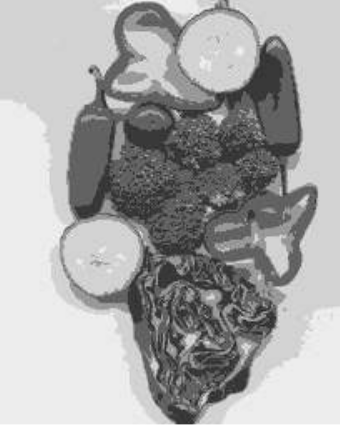
\includegraphics[width=0.48\textwidth]{img/ulearning/fruits_intensity}
		\caption{Clustering on pixels intensity.}
	\end{minipage}        
	\hspace{1.cm}
	\begin{minipage}[t]{0.5\linewidth} 
		\centering
		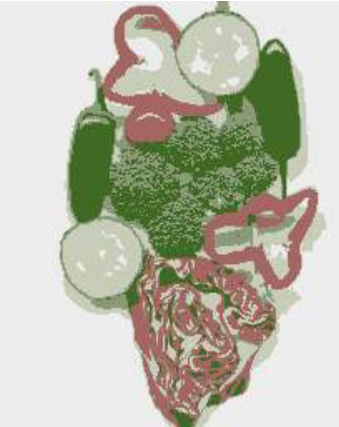
\includegraphics[width=0.48\textwidth]{img/ulearning/fruits_color}
		\caption{Clustering on pixels color.}
	\end{minipage}
\end{figure}
\FloatBarrier


\newpage
\section{K-Means}
K-Means is one of the simplest, famous and used iterative clustering algorithms. It aims to partition $n$ objects into $K$ maximal cohesive groups. The goal of the K-Means algorithm is to reach the following state: each observation belongs to the cluster with the nearest center. Its implementation can be shortly described in few lines:

\begin{itemize}
	\item \textbf{Initialization:} Pick $K$ random points as cluster centers (centroids).
	\image{img/ulearning/kmeans1}{Initialization with $K=2$.}{0.3}
	\item \textbf{Alternate:}
	\begin{enumerate}
		\item Assign data points to closest cluster centroid.
		\item For each cluster C update the corresponding centroid to the average of points in C.
		\begin{figure}[H]
			\begin{minipage}[t]{0.42\linewidth} 
				\centering
				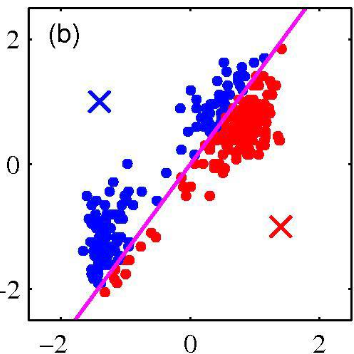
\includegraphics[width=0.68\textwidth]{img/ulearning/kmeans2}
				\caption{Iterative step 1.}
			\end{minipage}        
			\hspace{2.5cm}
			\begin{minipage}[t]{0.42\linewidth} 
				\centering
				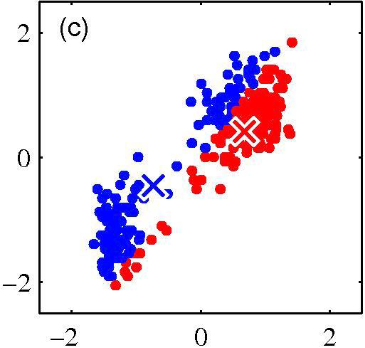
\includegraphics[width=0.68\textwidth]{img/ulearning/kmeans3}
				\caption{Iterative step 2.}
			\end{minipage}
		\end{figure}
		\FloatBarrier
	\end{enumerate}
	\item \textbf{Stop:} When no points' assignments change.
	\begin{figure}[H]
		\begin{minipage}[t]{0.42\linewidth} 
			\centering
			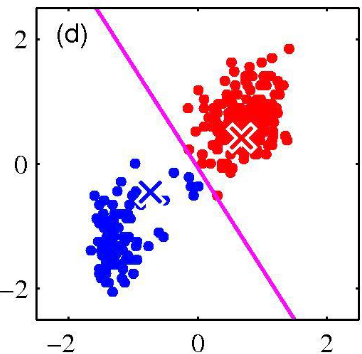
\includegraphics[width=0.68\textwidth]{img/ulearning/kmeans4}
			\caption{Repeat until convergence.}
		\end{minipage}        
		\hspace{2.5cm}
		\begin{minipage}[t]{0.42\linewidth} 
			\centering
			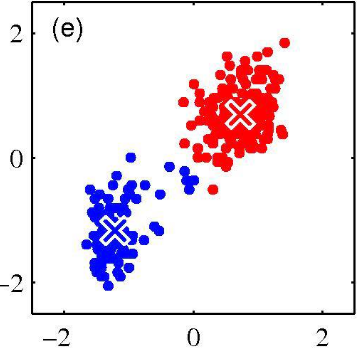
\includegraphics[width=0.68\textwidth]{img/ulearning/kmeans5}
			\caption{Final output.}
		\end{minipage}
	\end{figure}
\end{itemize}
\newpage
Formally speaking we can define the K-Means algorithm over the set of points $X$ in the following way:
\begin{enumerate}
	\begin{footnotesize}
	\item Initialize cluster centroids $\mu_1, \dots, \mu_k,$.
	\item Repeat until all points remain unchanged (convergence):
	\end{footnotesize}
		\begin{enumerate}[label*=\arabic*.]
			\item  $\forall i\in X \quad c^{(i)} = \arg\min_j \vert\vert x^{(i)}-\mu_j\vert\vert^2$
			\item $\forall j\in C \quad \mu_j = \frac{\sum_{i=1}^m 1\{c^{(i)} = j\}x^{(i)}}{\sum_{i=1}^m 1\{c^{(i)} = j\}}$
		\end{enumerate}
\end{enumerate}

\paragraph*{Properties of K-Means.} K-Means benefits of the following properties:
\begin{itemize}
	\item It is guaranteed to converge in a finite number of steps.
	\item It minimizes an objective function, which represents the compactness of the retrieved $K$ clusters:
	$$\arg \min_C\sum_{i=0}^K \Biggl\{ \sum_{j \in \text{elements of } C_i\text{ cluster}} ||x_j - \mu_i||^2 \Biggr\}$$
	where $\mu_i$ is the centroid of cluster $i$.
	\item It is a polynomial algorithm: $O(Kn)$ for assigning each sample to the closest cluster and $O(n)$ for the update of the clusters center.
\end{itemize}
It is possible to say that K-Means is a very simple and efficient method but, on the other hand, it is strongly sensible to the initialization phase. If the initial centroids are not chosen correctly the algorithm converges to a local minimum of the error function. Another disadvantage of K-Means is that does not work well in presence non-convex shapes. 


\section{Eigenvector-based Clustering}~\label{eingenvector-based-clustering}
The eigenvector-based clustering collects different techniques that use properties of eigenvalues and eigenvectors for solving the clustering problem.
Let us represent a cluster using a vector $x$ whose $k$-th entry captures the participation of node $k$ in that cluster. If a node does not participate in cluster $x$, the corresponding entry is zero. We also impose the restriction that $x^Tx = 1$. The goal of the clustering algorithm is to maximize:
\begin{equation}~\label{cohesiveness}
\arg\max_x \sum_{i=1}^n \sum_{j=1}^n w_{ij} x_i x_j = x^TAx
\end{equation}
which measures the cluster's cohesiveness and $x_i$, $x_j$ represent the measure of centrality to the cluster and it is defined as:
$$x_i = \begin{cases}
\neq 0 \text{  if } i \in C\\
= 0 \text{  if } i \notin C
\end{cases}$$.\\
Coming back to the notion of eigenvalues of a matrix we can say that $\lambda$ is an eigenvalue of $A$ and $x_\lambda$ is the corresponding eigenvector if:
$$Ax_\lambda = \lambda x_\lambda$$
From which we can derive that:
$$x_\lambda^TAx_\lambda = \lambda x_\lambda^Tx_\lambda = \lambda$$
There are two important theorems that defines the nature of eigenvalues of a $n\times n$ matrix $A$:
\begin{enumerate}
	\item If $A = A^T$ then $A$ is symmetric and has only "\textit{real}" eigenvalues. It means that we can sort them, from the smallest one to the largest one.
	\item If $A$ is symmetric then $\max_x x^TAx$ corresponds to the largest eigenvalue $\lambda$. Moreover, the corresponding eigenvector $x_\lambda$ is the argument which maximizes the cohesiveness.
\end{enumerate}
Taking advantage of the two theorems we can say that considering $A$ as the affinity matrix, then clustering problem \ref{cohesiveness} corresponds to an \textbf{eigenvalue problem}, maximized by the eigenvector of $A$ with the largest eigenvalue.\\

\paragraph*{Clustering by Eigenvectors Algorithm\\\\} 
We can define the algorithm for extracting clusters from data points using the eigenvectors strategy with the following steps:
\begin{enumerate}
	\begin{footnotesize}
	\item Construct the affinity matrix $A$ from input $G$.
	\item Compute the eigenvalues and eigenvectors of $A$.
	\item Repeat
	\item $\quad$ Take the largest unprocessed eigenvalue and the corresponding eigenvector.
	\item $\quad$ Zero all the components corresponding to samples that have already been clustered.
	\item $\quad$ Threshold the remaining components to detect which elements belong to this cluster.
	\item $\quad$ If all elements have been accounted for, there are sufficient clusters.
	\item Until there are sufficient clusters.
	\end{footnotesize}
\end{enumerate}

\subsection{Clustering as Graph Partitioning}
Let $G=(V,E,w)$ is an undirected weighted graph with $\vert V\vert$ nodes (samples) and $\vert E\vert$ edges. Note that it is undirected when the affinity matrix is symmetric. Given two graph partitions of vertices $A$ and $B$, with $B=V\setminus A$, we define cut$(A,B)$ in the following way:\\
$$cut(A,B) = \sum_{i \in A} \sum_{j \in B} w(i,j)$$
\image{img/ulearning/minCut}{Minimum cut problem.}{0.8}
In the MinCut problem, we look for the partitioning that minimizes the cost of crossing from one $A$ to $B$, which is the sum of weights of the edges which cross the cut. The fundamental idea is to consider the clustering problem as a graph partitioning. Indeed, the MinCut problem can be considered a good way of solving the clustering problem in graph data. The MinCut clustering is advantageous because it is solvable in polynomial time but, on the other hand, it favors highly unbalanced clusters (often with isolated vertices), indeed, it only measures what happens between the clusters and not what happens within the clusters.
\image{img/ulearning/minCut2}{Minimum cut unbalance clusters.\cite{normalized_cut}}{0.45}

\subsection{Normalized Cut}
In order to overcome the problem of unbalanced clusters, a normalized version of the min cut problem, called \textbf{Normalized Cut}, is used and it is defined by:\\

$$Ncut(A,B) = \underbrace{cut(A,B)}_{\text{Between A and B}}\left( \underbrace{\frac{1}{vol(A)} + \frac{1}{vol(B)}}_{\text{Within A and B}}\right)$$\\

where $vol(A)$ is the volume of the set $A$ given by $vol(A) = \sum_{i \in A}d_i,~A \subseteq V$ and $d_i = \sum_j w_{i,j}$ is the degree of nodes (sum of weights).\\
The Normalized Cut has the advantage of taking into consideration what happens within clusters, indeed, considering $vol(A)$ and $vol(B)$ it takes into account what's going on within $A$ and $B$.
\newpage

\subsection{Graph Laplacians}
From an accurate analysis \citeauthor{spectral_tutorial} discovered that the main tools for spectral clustering are graph Laplacian matrices, defined in the spectral graph theory.  In this section we are going to define different graph Laplacians and point out their most important properties since they will be later on used for solving the MinCut and NMinCut problem.

\paragraph{The Unnormalized Graph Laplacian.} The  \textbf{unnormalized graph Laplacian} matrix is defined as:
$$L = D - W$$

where:
\begin{itemize}
	\item $D$ is a diagonal matrix containing information about the degree of each node in $G$.
	\item $W$ is the affinity matrix of $G$, containing $1s$ or $0s$ if nodes are adjacent. Diagonal elements are all set to $0$.
\end{itemize}
In the following we provide an example of matrices $D$ and $W$ obtained considering the graph shown in Fig. \ref{fig:graphG}.
\begin{figure}[H]
	\begin{minipage}[t]{0.49\linewidth} 
		\centering
		$$ D = \begin{bmatrix}
		2 & 0 & 0 & 0 & 0 & 0 \\
		0 & 4 & 0 & 0 & 0 & 0 \\
		0 & 0 & 4 & 0 & 0 & 0 \\
		0 & 0 & 0 & 1 & 0 & 0 \\
		0 & 0 & 0 & 0 & 3 & 0 \\
		0 & 0 & 0 & 0 & 0 & 2 \\
		\end{bmatrix}$$
		\caption{Degree matrix $D$.}
	\end{minipage}        
	\hspace{1cm}
	\begin{minipage}[t]{0.49\linewidth} 
		\centering
		$$ W = \begin{bmatrix}
		0 & 1 & 1 & 0 & 0 & 0 \\
		1 & 0 & 1 & 1 & 1 & 0 \\
		1 & 1 & 0 & 0 & 1 & 1 \\
		0 & 1 & 0 & 0 & 0 & 0 \\
		0 & 1 & 1 & 0 & 0 & 1 \\
		0 & 0 & 1 & 0 & 1 & 0 \\
		\end{bmatrix}$$
		\caption{Affinity matrix $W$.}
	\end{minipage}
\end{figure}

The elements of $L$ are given by:
$$
L _ { i , j } = \left\{ \begin{array} { l l } { \operatorname { d } \left( v _ { i } \right) } & { \text { if } i = j } \\ 
{ - 1 } & { \text { if } i \neq j \text { and } v _ { i } \text { is adjacent to } v _ { j } } \\ 
{ 0 } & { \text { otherwise } } \end{array} \right.
$$
where $d(v_i)$ is the degree of the vertex $i$.
\imageLabel{img/ulearning/graphLaplacian}{Laplacian matrix L associated to the graph in the left.}{0.85}{graphG}

In \cite{spectral_tutorial} are reported the properties satisfied by the matrix $L$, that are:
\begin{enumerate}
	\item For all vectors $f$ in $\mathbb{R}^n$, we have:
	$$f ^ { \top } L f = \frac { 1 } { 2 } \sum _ { i, j = 1 } ^ { n } w _ { i j } \left( f _ { i } - f _ { j } \right) ^ { 2 }$$
	This is proved by the definition of $d_i$:
	$$\begin{aligned} 
	f ^ { \top } L f & = f ^ { \top } D f - f ^ { \top } W f = \sum _ { i=1 }^n d _ { i } f _ { i } ^ { 2 } - \sum _ { i , j =1 }^n f _ { i } f _ { j } w _ { i j } \\ 
	& = \frac { 1 } { 2 } \left( \sum _ { i=1 }^n \left( \sum _ { j=1 }^n w _ { i j } \right) f _ { i } ^ { 2 } - 2 \sum _ { i, j=1 }^n f _ { i } f _ { j } w _ { i j } + \sum _ { j=1 }^n \left( \sum _ { i=1 }^n w _ { i j } \right) f _ { j } ^ { 2 } \right) \\ 
	& = \frac { 1 } { 2 } \sum _ { i ,j=1 }^n w _ { i j } \left( f _ { i } - f _ { j } \right) ^ { 2 } 
	\end{aligned}$$
	
	\item $L$ is symmetric (by assumption) and positive semi-definite. The symmetry of $L$ follows directly from the symmetry of $W$ and $D$. The positive semi-definiteness is a direct consequence of the first property, which shows that 	$f ^ { T } L f \geq 0$
	
	\item The smallest eigenvalue of $L$ is 0, the corresponding eigenvector is the constant 1 vector.
	\item $L$ has $n$ non-negative, real-valued eigenvalues $0 = \lambda _ { 1 } \leq \lambda _ { 2 } \leq \ldots \leq \lambda _ { n }$
\end{enumerate}

First relation between spectrum and clusters:
\begin{itemize}
	\item The multiplicity of eigenvalue $\lambda_1=0$ corresponds to the number of connected components of the graph.
	\item The eigenspace is spanned by the characteristic function of these components (so all eigenvectors are piecewise constant).
\end{itemize}

\paragraph{Normalized Graph Laplacians.} In literature it is also defined the normalized form of a Laplacian graph. In particular, there exists two definitions that are closely related:
$$\begin{array} { l } { L _ { \mathrm { sym } } = D ^ { - 1 / 2 } L D ^ { - 1 / 2 } = I - D ^ { - 1 / 2 } W D ^ { - 1 / 2 } } \\ { L _ { \mathrm { rw } } = D ^ { - 1 } L = I - D ^ { - 1 } W } \end{array}$$
The first matrix $L_{sym}$ is a symmetric matrix, and the second one $L_{rw}$ as a normalized form of a Laplacian graph which is closely connected to a random walk \cite{spectral_tutorial}.

\begin{defn}[Properties for Laplacian matrices and normalized ones]{} In relation to Laplacian matrices, it is possible to notice that, let $L$ be the Laplacian of a graph $G=(V,E)$. Then, $L \geq 0$, indeed:\\
	$\forall x = (x_1, \dots, x_n),$
	$$\begin{aligned} x^{T}Lx &= x^{T} \sum_{e \in E} L_{e} x \\ &=\sum_{e \in E} x^T L_{e} x \\ &=\sum_{i, j \in E}\left(x_{i}-x_{j}\right)^{2} \geq 0 \end{aligned}$$
	In relation instead to the normalized Laplacian Matrix we have that:
	$$\forall x \in \mathbb{R}^n \quad x^TLx = \sum_{i,j} \left(\frac{x(i)}{\sqrt{d(i)}} - \frac{x(j)}{\sqrt{d(j)}} \right)^2 \geq 0$$
\end{defn}
\par \bigskip \bigskip \noindent


\subsection{Solving Ncut}~\label{solveNcutTheory}
Any cut $(A,B)$ can be represented by a binary indicator vector $x$:
$$x_i = \begin{cases}
+1 \text{  if } i \in A\\
-1 \text{  if } i \in B
\end{cases}$$
It can be shown that:
\begin{equation}~\label{solvencut}
min_x ~ Ncut(x) = min_y \underbrace{\frac{y'(D-W)y}{y'Dy}}_{\text{Rayleigh quotient}}
\end{equation}

subject to the constraint that $y ^ { \prime } D1 = \sum_{i} y_{i} d _ { i } = 0$ (with $y _ { i } \in \{ 1 , - b \}$ (relaxation introducing also real values), indeed $y$ is an indicator vector with 1 in the $i$-th position if the $i$-th feature point belongs to $A$, negative constant ($-b$) otherwise).

\begin{thm}[Solving Ncut proof]{}
	$$\lambda_2 = \min_x \frac{x^TLx}{x^Tx} = \min_x \frac{x^TD^{-1/2}LD^{-1/2}x}{x^Tx} \qquad \text{Remember } L_{sym} = D^{-1/2}LD^{-1/2}$$
	\text{Considering the change of variables obtained by setting} $y=D^{-1/2}x$ \text{ and } $x = D^{1/2}y$:
	$$\lambda_2 = \min_y \frac{y^TLy}{(D^{1/2}y)^T(D^{1/2}y)} = \min_y \frac{y^TLy}{y^TDy}$$
\end{thm}

Issues rise up because solving Problem \ref{solvencut} is not computationally efficient since it is an \textbf{NP-Hard} problem. The huge Ncut time complexity brings us to take into consideration an approximation of it. If we relax the constraint that $y$ must be a discrete-valued vector and allow it to take on real values, then the original problem
$$\min _ { y } \frac { y ^ { \prime } ( D - W ) y } { y ^ { \prime } D y }$$
is equivalent to:
$$\min _ { y } y ^ { \prime } ( D - W ) y \quad \text { subject to } y ^ { \prime } D y = 1$$
This amount to solve a \textit{generalized} eigenvalue problem, but now the optimal solution is provided by the second smallest eigenvalue since we want to minimize the cut. Note that we pick the second smaller eigenvalues since we have seen the smallest one is always zero and corresponds to the trivial partitioning $A=V$ and $B=\emptyset$.
$$\underbrace{(D-W)}_{Laplacian}y=\lambda D y$$
We started from an NP-Hard problem and through relaxation we reached a feasible solution. However, we have not the warranty that the relaxed solution is in one to one correspondence.
\paragraph*{The effect of relaxation.} Through the relaxation we loose some precision in the final solution. 
\imageb{img/ulearning/relaxation1}{0.8}
Note that the original problem returns binary values $(-1,1)$, indicating the clustering membership. The relaxed version, on the right, returns continuous values of it can be the case that some points are not so clear to assign (close to the margin between the two). For that reason relaxed solution not always is in one-to-one correspondence with the original problem.

\subsection{Random Walk Interpretation} 
The Ncut problem can be formalized also in terms of random walk, as highlighted in \cite{spectral_tutorial}, since we want to find a cut that reduces the probability of jumping between nodes of different clusters. It can be defined by a  Markov chain where each data point is a state, connected to all other states with some probability. With our affinity $W$ and degree $D$, the stochastic matrix is:
$$P=D^{-1}W$$
which is the row-normalized version of $W$, so each entry $P(i,j)$ is a probability of "\textit{walking}" to state $j$ from state  $i$\cite{randomwalk_spectral}.
\imageb{img/ulearning/randomWalk}{0.20}
Probability of a walk through states $( s _ { 1 } , \dots , s _ { m })$ is given by:
$$P \left( s _ { 1 } , \ldots , s _ { 2 } \right) = P \left( s _ { 1 } \right) \prod _ { i = 2 } ^ { m } P \left( s _ { i } , s _ { i - 1 } \right)$$
Suppose we divide the states into two groups, and we want to minimize the probability of jumping between the two groups. We can formulate this as an eigenvector problem:
$$P y = \lambda y$$
where the component of vector $y$ will give the segmentation.\\
We can precise also that:
\begin{itemize}
	\item $P$ is a stochastic matrix.
	\item The largest eigenvalue is 1, and its eigenvector is the all-one vector 1. Not very informative about segmentation.
	\item The second largest eigenvector is orthogonal to the first, and its components indicate the strongly connected sets of states.
	\item Meila and Shi (2001) showed that minimizing the probability of jumping between two groups in the Markov chain is equivalent to minimizing Ncut.
\end{itemize}
\begin{thm}[Random Walk Proposition] $(\lambda, y)$ is a solution to $Py = \lambda y$ if and only if \footnote{Adapted from Y. Weiss}:
	\begin{itemize}
		\item $1-\lambda$ is an eigenvalue of $(D-W)y = \lambda D y$
		\item $y$ is an eigenvector of $(D-W)y = \lambda Dy$
	\end{itemize} 
	\textbf{Proof:}
	$$\begin{array} { l l } { P y = \lambda y } & { \Leftrightarrow \quad - P y = - \lambda y } \\
	{ } & { \Leftrightarrow \quad y - P y = y - \lambda y } \\
	{ } & { \Leftrightarrow \quad ( I - P ) y = ( 1 - \lambda ) I y } \\
	{ } & { \Leftrightarrow \quad \left( D ^ { - 1 } D - D ^ { - 1 } W \right) y = ( 1 - \lambda ) D ^ { - 1 } D y } \\
	{ } & { \Leftrightarrow \quad D ^ { - 1 } ( D - W ) y = D ^ { - 1 } ( 1 - \lambda ) D y } \\
	{ } & { \Leftrightarrow \quad ( D - W ) y = ( 1 - \lambda ) D y } \end{array}$$
\end{thm}
The problem is to find a cut $(A,B)$ in a graph $G$ such that a random walk does not have many opportunities to jump between the two clusters.\\
This is equivalent to the Ncut problem due to the following relation:
$$Ncut(A,B) = P(A|B) + P(B|A)$$
\subsection{2-way Ncut clustering algorithm}
In section \ref{solveNcutTheory} we have seen how to solve the Normalized Cut clustering problem, and here we want to discuss its implementation for extracting just two clusters:
\begin{enumerate}
	\begin{footnotesize}
	\item Compute the affinity matrix $W$, compute the degree matrix $D$. $D$ is diagonal and \\$D_{i,i} = \sum_{j \in V} W_{i,j}$
	\item Solve the generalized eigenvalue problem $(D-W)y = \lambda Dy$
	\item Use the eigenvector associated to the second smallest eigenvalue to bipartition the graph into two parts.
	\end{footnotesize}
\end{enumerate}
Sometimes there's not a clear threshold to split based on the second vector since it takes continuous values. In which way it is possible to choose the splitting point?
\begin{itemize}

	\item Pick a constant value (0 or 0.5).
	\item Pick the median value as the splitting point.
	\item Look for the splitting point that has minimum Ncut value:
	\begin{enumerate}
		\item Choose $n$ possible splitting points.
		\item Compute Ncut value.
		\item Pick the minimum.
	\end{enumerate}

\end{itemize}

\subsection{K-way Ncut clustering algorithm}
In the case we want to extract more than 2 clusters we can adopt two possible strategies:
\paragraph*{Approach \# 1.} It is a recursive two-way cuts:
\begin{enumerate}
	\begin{footnotesize}
	\item Given a weighted graph $G=(V,E,w)$, summarize the information into matrices $W$ and $D$.
	\item Solve $(D-W)y = \lambda Dy$ for eigenvectors with the smallest eigenvalues.
	\item Use the eigenvector with the second smallest eigenvalue to bipartition the graph by finding the splitting point such that Ncut is minimized.
	\item Decide if the current partition should be subdivided by checking the stability of the cut, and make sure Ncut is below the prespecified value.
	\item Recursively repartition the segmented parts if necessary.
	\end{footnotesize}
\end{enumerate}
Note that the approach is computationally wasteful, only the second eigenvector is used, whereas the next few small eigenvectors also contain useful partitioning information.

\paragraph*{Approach \#2.} Using the first $k$ eigenvectors:
\begin{enumerate}
	\begin{footnotesize}
	\item Construct a similarity graph and compute the unnormalized graph Laplacian $L$.
	\item Compute the $k$ smallest \textbf{generalized} eigenvectors $u _ { 1 } , u _ { 2 } , \dots , u _ { k }$ of the generalized eigenproblem $L u = \lambda D u$.
	\item Let $U = \left[ u_1, u_{ 2 }, \dots, u_{ k } \right] \in \mathbb { R } ^ { n \times k }$.
	\item Let $y_i \in \mathbb{ R }^k$ be the vector corresponding to the $i$th row of $U$.
	$$U = \left[ \begin{array} { c c c c } { u _ { 11 } } & { u _ { 12 } } & { \cdots } & { u _ { 1 k } } \\ { u _ { 21 } } & { u _ { 22 } } & { \cdots } & { u _ { 2 k } } \\ { \vdots } & { \vdots } & { \ddots } & { \vdots } \\ { u _ { n 1 } } & { u _ { n 2 } } & { \cdots } & { u _ { n k } } \end{array} \right] = \left[ \begin{array} { c } { y _ { 1 } ^ { T } } \\ { y _ { 2 } ^ { T } } \\ { \vdots } \\ { y _ { n } ^ { T } } \end{array} \right]$$
	\item Thinking of $y_i$'s as points in $\mathbb{ R }^k$, cluster them with $k$-means algorithms.
	\end{footnotesize}
\end{enumerate}

\subsection{Spectral Clustering vs $K$-Means}
First of all, let us define the spectral clustering algorithm \cite{spectral_algorithm}, its goal is to cluster objects that are connected but not necessarily compact or clustered within convex boundaries. The algorithm has in input the similarity matrix $S \in \mathbb{ R }^{n \times n}$ and the $k$ number of clusters to construct. It returns in output the $k$ clusters. It follows these steps:
\begin{enumerate}
	\begin{footnotesize}
	\item Construct a similarity graph and compute the normalized graph Laplacian $L_{sym}$.
	\item Embed data points in a low-dimensional space (spectral embedding), in which the clusters are more obvious, computing the $k$ smallest eigenvectors $v_1, \dots, v_k$ of $L_{sym}$. 
	\item Let $V=\left[v_1,\dots, v_k \right] \in \mathbb{ R }^{n \times k}$.
	\item Form the matrix $U \in \mathbb{ R }^{n \times k}$ from $V$ by normalizing the row sums to have norm 1, that is: 
	$$u_ { i j } = \frac { v _ { i j } } { \left( \sum _ { k } v _ { i k } ^ { 2 } \right) ^ { 1 / 2 } }$$
	\item For $i=1,\dots, n$, let $y _ { i } \in \mathbb { R } ^ { k }$ be the vector corresponding to the $i$th row of $U$.
	\item Cluster the points $y_i$ with $i=1,\dots,n$ with the $k$-means algorithm into clusters $C_1, \dots, C_k$.
	\end{footnotesize}
\end{enumerate}
Applying $k$-means to Laplacian eigenvectors allows us to find cluster with non-convex boundaries.
\imageb{img/ulearning/spectral1}{0.95}
\imageb{img/ulearning/spectral2}{0.95}
\imageb{img/ulearning/spectral3}{0.95}
One of the possible problems that could appear on the usage of the Spectral Clustering algorithm consists on choosing the best $k$. We want to find a $k$ such that all eigenvalues $\lambda_1, \dots, \lambda_k$ are very small, but $\lambda_{k+1}$ is relatively large. In this way, the choosing of $k$ maximizes the eigengap (difference between consecutive eigenvalues) $\delta_k = |\lambda_k - \lambda_{k-1}|$.
\imageb{img/ulearning/eigengap}{0.95}
\newpage

\section{Dominant Sets}
In the previous sections we have seen that data can be represented using weighted graphs, also called similarity graphs, in which data are represented by nodes in the graph and the edges represent the similarity relation between nodes. This representation allows us to codify also very complex structured entities.
In literature some authors argue to the fact that a cluster can be seen as a \textbf{maximal clique}\footnote{A \textbf{clique} is a subset of mutually adjacent vertices.\\ A \textbf{maximal clique} is a clique that is not contained in a larger one.} of a graph, indeed the concept of clique is related to the internal cluster criteria, instead maximal clique responds to the external criteria. But the standard definition of click does not consider weighted graphs. For this reason, dominant set is introduced by \citeauthor{dominantset} as an extension of the maximal clique problem. We are going to see that the notion of dominant set provides measures of cohesiveness of a cluster and vertex participation of different clusters.

\subsection{Cluster in Graph Theory}
Data to be clustered could be coded as an undirected weighted graph with no self-loops: $G=(V, E, \omega)$, where $V=\{1,\dots,n\}$ is the vertex set, $E\subseteq V\times V$ is the edges set and $w: E\rightarrow \mathbb{R}^*_+$ is the positive weight function. Vertices represent data points, edges neighborhood relationships and edge-weights similarity relations. $G$ is then represented with an adjacency matrix $A$, such that $a_{ij} = \omega(i,j)$. Since there are not self-loops we have that $\omega(i,i) = 0$ (main diagonal equal to $0$).\\
One of the key problem of clustering is that there is not a unique and well define definition of cluster, but in literature researches agree that a cluster should satisfy two conditions:
\begin{itemize}
	\item \textbf{High internal homogeneity}, also named \textit{Internal criterion}. It means that all the objects inside a cluster should be highly similar(or low distance) to each other.
	\item \textbf{High external in-homogeneity}, also named \textit{External criterion}. It means that objects coming from different clusters have low similarity (or high distance).
\end{itemize}
The idea of the criterion is that clusters are groups of objects which are strongly similar to each other if they become to the same cluster, otherwise they have a highly dissimilarity. 
Informally speaking a cluster is a set of entities which are alike, and entities from different clusters are not alike.

Let $S\subseteq V$ be a nonempty subset of vertices and $i \in S$. The average weighted degree of $i$ with regard to $S$ is defined as:\\
\begin{equation}
\text{awdeg}_S(i)=\frac{1}{|S|}\sum_{j\in S}a_{ij}
\end{equation}
This quantity over here represents the average similarity between entity $i$ and the rest of the entities in $S$. In other words how much similar $i$ is in average with all the objects in $S$.
It can be observed that $\text{awdeg}_{\{i\}}(i) = 0$  $\forall i \in V$, since we have no self-loops.\\
We now introduce a new quantity $\phi$ such that if $j \notin S$:
\begin{equation}
\phi_S(i, j)=a_{ij}-\text{awdeg}_S(i)
\end{equation}
Note that $\phi_{\{i\}}(i, j)=a_{ij}$ $\forall i, j\in V$ with $i \neq j$. $\phi_S(i, j)$ measures the relative similarity between $i$ and $j$ with respect to the average similarity between $i$ and its neighbors in $S$. This measures can be either positive or negative.

\begin{defn}[\citeauthor{ds1}, Node's weight]{}
Let $S\subseteq V$ be a nonempty subset of vertices and $i \in S$. The weight of $i$ with regard to $S$ is:
\begin{equation}
w_S(i)= \begin{cases}
1 & \text{if } |S| = 1 \\
\sum\limits_{j\in S\setminus \{i\}}\phi_{S\setminus \{i\}}(j, i)w_{S\setminus \{i\}}(j) & \text{otherwise}
\end{cases}
\end{equation}
\end{defn}

Further, the total weight of $S$ is defined to be $W(S)=\sum_{i\in S}w_S(i)$.
\image{img/ulearning/ws.png}{Weight of i respect to elements in S.}{0.18}
Note that $w_{\{i, j\}}(i)=w_{\{i, j\}}(j)=a_{ij}$ $\forall i, j \in V \land i\neq j$. Then, $w_S(i)$ is calculated simply as a function of the weights on the edges of the sub-graph induced by $S$.\\

Intuitively, $w_S(i)$ gives a measure of the similarity between $i$ and $S\setminus \{i\}$ with respect to the overall similarity among the vertices of $S\setminus \{i\}$. In other words, how similar (important) $i$ is with respect to the entities in $S$.
An important property of this definition is that it induces a sort of natural ranking among vertices of the graph. 


\imageLabel{img/ulearning/graph.png}{Similarity graph example.}{0.15}{gex}

Considering the graph proposed in Figure \ref{fig:gex}, we can derive a ranking between nodes: $$w_{\{1,2,3\}}(1) < w_{\{1,2,3\}}(2) < w_{\{1,2,3\}}(3)$$
\begin{defn}[\citeauthor{ds1}, Dominant Set]{} A nonempty subset of vertices $S\subset V$ such that $W(T)>0$ for any nonempty $T \subseteq S$, is said to be a \textbf{dominant set} if:
\begin{itemize}
	\item $w_S(i) > 0$ $\forall i \in S \qquad$ (\textit{internal homogeneity})
	\item $w_{S \cup \{i\}}(i) < 0$ $\forall i \notin S \qquad$ (\textit{external homogeneity})
\end{itemize}
\end{defn}
These conditions correspond to cluster properties (\textbf{internal homogeneity} and \textbf{external in-homogeneity}). Informally we can say that the first condition requires that all the nodes in the cluster $S$ are important (high weight, similar). The second one assumes that if we consider a new point in the cluster $S$, the cluster cohesiveness will be lower, meaning that the current cluster is already maximal.\\
By definition, dominant sets are expected to capture compact structures. Moreover, this definition is equivalent to the one of maximal clique problem when applied to unweighted graphs.
\image{img/ulearning/dominant_def}{The set \{1,2,3\} is dominant.}{0.2}


\subsection{Link to Standard Quadratic Optimization}
Clusters are commonly represented as an $n$-dimensional vector expressing the participation of each node to a cluster. Large numbers denote a strong participation, while zero values no participation. In section \ref{eingenvector-based-clustering} we have seen that the goal of clustering algorithm is to maximize the cohesiveness of the retrieved clusters. Formally speaking the goal can be expressed using the following optimization problem:
\begin{equation}\label{SPQ}
\begin{array}{lcl}
\text{maximize} & f(x) \\
\text{subject to} & x \in \Delta
\end{array}
\end{equation}
where $A$ is a symmetric real-valued matrix with null diagonal and \begin{equation}
\Delta=\{x\in\mathbb{R}^n:x\geq 0 \land e^\top x = 1\}
\end{equation} is the standard simple of $\mathbb{R}^n$. This yields the following standard quadratic problem in which local solution corresponds to a maximally cohesive cluster.

The entity $x$ is a strict local solution of problem \ref{SPQ} if there exists a neighborhood $U \subset	\Delta$ of $x$ such that $f(x) > f(z)$ $\forall z \in U\setminus\{x\}$. Then we define the support $\sigma(x)$ of $x\in\Delta$ as the index set of the positive components in $x$.
$$\sigma(x) = \{i\in V: x_i > 0\}$$
In other words $\sigma(x)$ is the set of vertices in $V$ that belongs to the extracted cluster.

\begin{defn}[\citeauthor{dominantset}, Characteristic vector]{}~\label{ds_simplex} A non-empty subset $C \subseteq V$ and $C$ is a dominant set, admits a weighted \textbf{characteristic vector} $x^c\in \Delta$ if it has positive total weight $W(C)$, in which:

$$
x_i^C= \begin{cases}
\frac{W_c(i)}{W(C)} & \text{if } i\in C\\
0 & \text{otherwise}
\end{cases}
$$
\end{defn}
The important notion provided by Definition \ref{ds_simplex} is that also dominant set solutions belong to the standard simplex, as imposed in problem \ref{SPQ}. The advantage is that, empirically, strict local maximizers of the dominant sets procedure work well in extracting clusters.


\subsection{Link to Game Theory}
Game theory is a theoretical framework used for examining and analyzing models of strategic interaction between competing rational actors. The clustering problem, as suggested by \citeauthor{dominantset}, 
can be formulated in terms of a game, also called \textit{clustering game}, with the following properties:
\begin{itemize}
	\item \textbf{Symmetric game}, the payoff of playing any strategy does not depend by the player but only by the strategy itself.
	
	\item \textbf{Complete knowledge}, players have complete knowledge about the game, they know what are the strategies that can be played and the corresponding payoffs.
	
	\item \textbf{Non-cooperative game}, players take independent decisions about the strategy to play, they don't make a priori alliance.
	
	\item Players play only \textbf{pure strategies}, meaning that they do not behave “rationally” but they take decisions in a pre-programmed pattern.
\end{itemize}
In the clustering game we have two players that want to extract the best structure of cluster from data samples. The pure strategies available to the players are the data points themselves in $V$ and the similarity matrix $A$ is used as the \textit{payoff matrix} for the clustering game. The values $A_{ij}$ and $A_{ji}$ are the revenues obtained by player 1 and player 2 considering that they have player strategies $(i,j) \in V\times V$. Remember that the main diagonal of the similarity matrix is zero, meaning that $A_{ii}=0$.
A \textit{mixed strategy} $x=(x_1, \dots, x_n)^T \in \Delta$ is a probability distribution over the set of pure strategies, which models a stochastic playing strategy of a player. If player 1 and 2 play mixed strategies $(x_1, x_2) \in \Delta \times \Delta$, then the expected payoffs for the players are: $\mathbf{x_1^TAx_2}$ and $\mathbf{x_2^TAx_1}$ respectively.
The goal of the two players of course is to maximize as much as possible their resulting revenue. During the game each player extract an object $(i,j)$ and the resulting revenue is associated according to the payoff matrix $A$. Since we are considering $A$ equal to the similarity matrix we can say that in order to maximize their revenue the two players would coordinate their strategies so that the extracted samples belong to the same cluster. In other words, only by selecting objects belonging to the same cluster, each player is able to maximize his expected payoff. The desired condition is that the two players reach a \textbf{symmetric Nash equilibrium}, that is state in which the two players agree about the cluster membership. A \textbf{Nash Equilibrium} is a mixed-strategy profile $(x_1,x_2)\in \Delta\times \Delta$ such that no player can improve the expected payoff by changing his playing strategy, given the opponent's strategy being fixed. This concept can be expressed with the following expression:\\
$$y_1^TAx_2 \leq x_1^TAx_2 \qquad y_2^TAx_1 \leq x_2^TAx_1 \qquad \forall (y_1,y_2) \in (V\times V).$$ 
A Nash equilibrium is \textbf{symmetric} if $x_1 = x_2$, meaning that considering a symmetric Nash Equilibrium $x \in \Delta$ the two conditions hold in a unique one:\\
$$y^TAx \leq x^TAx$$

The symmetric Nash equilibrium condition satisfies the internal homogeneity criterion required by the dominant set definition. However, it does not include any kind of constraint that guarantees the maximality condition. In order to satisfy this condition it is necessary to look for a different type of Nash Equilibrium, known as \textbf{Evolutionary Stable Strategy (ESS)}. 

\paragraph{Definition.} A symmetric Nash equilibrium $x\in \Delta$ is an ESS if it satisfies also:
$$y^TAx = x^TAx \implies x^TAy > y^TAy \qquad \forall y \in \Delta\setminus\{x\}$$

$$y^TAx = x^TAx \implies x^TAy < x^TAx \qquad \forall y \in \Delta\setminus\{x\}$$
Even if the strategy $y$ provides the same payoff of the strategy $x$, it is better to play $x$ since the payoff against itself is greater than the one provided by $y$. The two strategies $x$ and $y$ represents two Nash Equilibrium, but only $x$ is an ESS.\\
In conclusion we can say that the ESSs of the clustering game with affinity matrix $A$ are in \textbf{correspondence} with dominant sets of the same clustering problem instance. However, we can also conclude that ESS’s are in one-to-one correspondence to (strict) local solutions of StQP.\\
It is possible to say that ESS's satisfy the main characteristics of a cluster:
\begin{itemize}
	\item \textbf{Internal coherency:} High support for all samples within the group.
	\item \textbf{External incoherency:} Low support for external samples.
\end{itemize}


\subsection{Extracting Dominant Sets}
One of the major advantages of using dominant sets is that it can be written with few lines of code, and moreover we can define different clustering approaches:
\begin{itemize}
	\item Extracting a dominant set, done using the replicator dynamics procedure.
	\item Partitioning of the data points, obtained using the \textit{peel-off} strategy, which means that at each iteration we extract a dominant set and the corresponding vertices are remove from the graphs. This is done until all vertices have been clustered (Partitioning-based clustering).
	\item Extracting overlapping clusters, obtained enumerating dominant sets. 
\end{itemize}
In our applications we are going to deal with the second one, assuming that each entity belongs to a cluster. This assumption is required since the subject of this thesis is based on comparing three algorithms, but the first two (K-Means  and Spectral clustering) are essentially partitioning-based algorithm.\\

The \textbf{Replicator Dynamics}  are deterministic game dynamics that have been developed in evolutionary game theory. It considers an ideal scenario whereby individuals are repeatedly drawn at random from a large, ideally infinite, population to play a two-player game. Players are not supposed to behave rationally, but they act according to an inherited behavioral pattern (pure strategy). An evolutionary selection process operates over time on the distribution of behaviors \cite{replicator}.\\

Let $x_i(t)$ the population share playing pure strategy $i$ at time $t$. The state of the population at time $t$ is: $x(t) = (x_1(t),\dots,x_n(t))\in\Delta$.\\
We define an evolution equation, derived from Darwin's principle of nature selection:
$$\dot{x_i} = x_i~g_i(x)$$

where $g_i$ specifies the rate at which pure strategy $i$ replicates, $\dot{x_i}$ is grow rate of strategy $i$. 
$$\frac{\dot{x_i}}{x_i} \propto \text{payoff of pure strategy }i\text{ - average population payoff}$$
The most general continuous form is given by the following equation:
$$\dot{x_i} = x_i[(Ax)_i - x^TAx]$$
where $(Ax)_i$ is the $i$-th component of the vector and $x^TAx$ is the average payoff for the population. If we have a result better than the average strategy there's an improvement.

\begin{thm}[Nachbar,1990 TaylorandJonker,1978]{}
A point $x\in\Delta$ is a Nash equilibrium if and only if $x$ is the limit point of a replicator dynamics trajectory starting from the interior of $\Delta$. Furthermore, if $x\in\Delta$ is an ESS, then it is an asymptotically stable equilibrium point for the replicator dynamics.\\
\end{thm}

Assuming that the payoff matrix $A$ is symmetric $(A = A^T)$ then the game is said to be doubly symmetric. Thanks to this assumption we can derive some conclusions:
\begin{itemize}
	\item \textit{Fundamental Theorem of Natural Selection (Losert and Akin,1983)} \\
	For any doubly symmetric game, the average population payoff $f(x) = x^TAx$ is strictly increasing along any non-constant trajectory of replicator dynamics, meaning that $\frac{df(x(t))}{dt} \geq 0$ $\forall t \geq0$, with equality if and only if $x(t)$ is a stationary point.
	
	\item \textit{Characterization of ESS's (Hofbauer and Sigmund, 1988)}\\
	For any doubly symmetric game with payoff matrix $A$, the following statements are equivalent:
	\begin{itemize}
		\item $x\in \Delta^{ESS}$
		\item $x \in \Delta$ is a strict local maximizer of $f(x) = x^TAx$ over the standard simplex $\Delta$.
		\item $x\in\Delta$ is asymptotically stable in the replicator dynamics.
	\end{itemize}
\end{itemize}


A well-known discretization of replicator dynamics, which assumes non-overlapping generations, is the following (assuming a non-negative $A$): 
$$
x_i(t+1) = x_i(t)\frac{A(x(t))_i}{x(t)^TAx(t)}
$$
which inherits most of the dynamical properties of its continuous-time counterpart.
\image{img/ulearning/rep_dynamics}{MATLAB implementation of discrete-time replicator dynamics}{0.5}
The components of the converged vector give us a measure of the participation of the corresponding vertices in the cluster, while the value of the objective function provides of the cohesiveness of the cluster.

\subsection{Dominant Sets Hierarchy}
A useful extension of the Dominant Sets formulation is introduced in the optimization problem. The new formulation is now defined:
\begin{equation}\label{alphaSPQ}
\begin{array}{lcl}
\text{maximize} & f_\alpha(x) = x^\prime(A - \alpha I)x\\
\text{subject to} & x \in \Delta
\end{array}
\end{equation}
where $\alpha \geq 0$ is a parameter and $I$ is the identity matrix.\\

The parameter $\alpha$ affects the number of clusters found by the algorithm. With an huge value of $\alpha$ each point defines a cluster since we require a strong cohesiveness. Instead decreasing the value of $\alpha$ the number of cluster increases.\\
The objective function $f_{\alpha}$ has now two kinds of solutions:
\begin{itemize}
	\item solutions which correspond to dominant sets for original matrix $A$ $(\alpha=0)$.
	
	\item solutions which don't correspond to any dominant set for the original matrix $A$, although they are dominant for the scaled matrix $A+\alpha(ee' - I)$. In other words, it allows to find subsets of points that are not sufficiently coherent to be dominant with respect to $A$, and hence they should be split.	
\end{itemize}
This algorithm has the basic idea of starting with a sufficiently large $\alpha$ and adaptively decrease it during the clustering process following these steps:
\begin{enumerate}
	\item Let $\alpha$ be a large positive value (ex: $\alpha > |V|-1$).
	\item Find a partition of the data into $\alpha$-clusters.
	\item For all the $\alpha$-clusters that are not 0-clusters recursively repeat step 2 with decreasing $\alpha$.
\end{enumerate}
\newpage
\subsection{Properties}
\begin{itemize}
	\item \textbf{Well separation between structure and noise.} In such situations it is often more important to cluster a small subset of the data very well, rather than optimizing a clustering criterion over all the data points, particularly in application scenarios where a large amount of noisy data is encountered. 
	
	\item \textbf{Overlapping clustering}. In some cases we can have that two distinct clusters share some points, but partitional approaches impose that each element cannot be long to more than one cluster.
	
	\item Dominant sets can be found by mining \textbf{local solutions}, so it is not necessary to look for global solutions.
	
	\item Deal very well in presence of noise.
	
	\item Strong connection with theoretical results.
	
	\item Makes no assumptions on the structure of the affinity matrix, being it able to work with asymmetric and even negative similarity functions.
	
	\item Does not require a priori knowledge on the number of clusters (since it extracts them sequentially).
	
	\item Leaves clutter elements unassigned (useful, e.g., in figure/ground separation or one-class clustering problems).
	
	\item Limiting the number of dynamic's iterations it is possible to detect quasi-click structures.
\end{itemize}


	%\include{crafting_advExamples} ask to the author
	%\include{results}
	\chapter{Conclusions and Future Work}~\label{conclusioni}
In this work, we have presented how adversarial machine learning is increasingly attracting researchers and privates due to the strong implications that it can have in real life. We have shown how in sophisticated domains, such as cyber-security, adversarial perturbations can bring to dangerous conclusions. We have in particular analyzed the impact of adversarial machine learning for the unsupervised paradigm. 
After having shortly reviewed image segmentation in terms of clustering, we have noted how fooling an image segmentation algorithm can bring sophisticated systems to make dangerous decisions. \\
We have testified a lack of adversarial analysis in clustering algorithms and we have addressed this lack by performing extensive experimentation on three clustering algorithms, discovering a strong sensitivity to the adversarial perturbations. In particular, we have developed three methods for crafting adversarial examples against K-Means, Spectral and Dominant Sets clustering. The first two methods have been designed for fooling image segmentation algorithms, and we have discussed how they work along with the differences between them. The last one, instead, has been designed for fooling feature-based data clustering.
We have shown how the three clustering algorithms behave, for both applications, in presence of adversarial noise. In particular, we have seen how Spectral Clustering seems to be strongly sensitive to small perturbations with respect to the other two clustering algorithms. Moreover, we have seen how K-Means and Dominant Sets preserve a similar behavior against adversarial noise, but the latter has the advantage of working better in absence of adversarial noise.\\
During the development of this work we have realized some ideas that could be interesting to address in the future. The first one is related to the optimization of the adversarial algorithms. At the moment, the major component that results to be computationally costly is the noise evaluation, which requires multiple iterations of the clustering algorithms. A possible solution could be to develop the proposed clustering algorithms in order to work with GPUs, to speed up the computations. In our implementation the designed code is strongly scalable, meaning that it is possible to run the entire algorithm over parallel architectures without much effort. Right now, due to the absence of GPU-supported implementations of clustering algorithms, we can not run the adversarial algorithms on GPUs. Another idea for speeding up the adversarial target algorithm \ref{alg:target_clustering}, is to introduce a new heuristic that avoids the injection of noise if the target samples are locally close to the desired cluster. Indeed, at the moment target samples are always moved towards the destination cluster, meaning that the algorithm injects small perturbations even if samples are already locally close. From multiple observations, we have seen that the optimizer leaves local features more or less unchanged if samples are locally close. This consideration brings us to the conclusion that executing the optimization for those features can lead to waste computational resources, since only negligible perturbations are crafted.\\
The second topic of interest for future work is the connection between adversarial examples crafted against clustering and supervised classification models. A clustering algorithm can be seen as a way for estimating probability distributions of samples. If samples belong to the same group, then they are probably sampled from the same distribution. We believe that fooling clustering is tightly related to change the classes probability distributions. Supervised models are built with the goal of discriminating samples coming from different classes, therefore we think that adversarial examples crafted to fool clustering can even fool supervised algorithms. If we could verify the correctness of this idea then we might think to use the adversarial masks, like in Fig. \ref{noiseMaskOptimal}, generated offline against clustering algorithms, for fooling online classifiers. This strategy could be interesting for drastically reducing the computational time required for crafting adversarial examples. 
%To the best of our knowledge, nowadays we require to optimize each sample --e.g. an image-- independently, in order to craft adversarial samples against classifiers. This strategy can be adopted against offline applications, or time invariant inputs. Conversely, for videos data, given that consecutive frames come from the same distribution, we think that crafting a generic adversarial mask can be sufficient for fooling multiple consecutive frames, strongly reducing the computational costs.\\
The latest idea is related to the design of the target clustering algorithm \ref{alg:target_clustering}. Indeed, it works moving samples from one cluster towards another one. We can imagine to generalize this framework allowing the attacker to move samples from a cluster towards multiple ones.\\
%We hope that with our contributions can invoke attentions from related researchers and practitioners, who
%would include security analysis in the application or development of clustering algorithms.



%K-Means again result to be more robust then then the others, but this is probably related to the fact the we are using similarities based on the distances. It could be reasonable in the future to expand this analysis introducing other similarity measures.

	
	
	\bibliographystyle{plainnat}
	{\footnotesize
		\bibliography{bibliography}
	}
	
	
\end{document}
